\chapter{系统实现}

本章基于上一章的需求分析及概要设计,介绍系统各个模块的详细设计及具体实现。我们通过
用例图、流程图、类图等方式来展示系统模块的功能及交互关系。

\section{模块化设计}

一般用户在登录后可以上传视频并进行编辑、查询与管理编辑结果,并且可以查看开发者的相关信息。用户用例图如~\ref{fig:user-uml}所示。
\begin{figure}[ht]
    \centering
    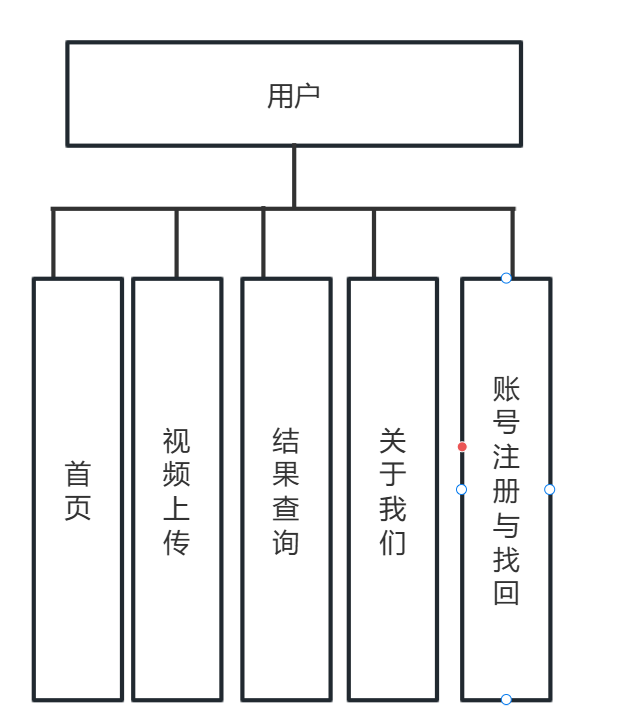
\includegraphics[width=0.3\textwidth]{source/img/user_uml.png}
    \bicaption{用户用例图}{User Use Case Diagram}
    \label{fig:user-uml}
\end{figure}
管理员用户除了一般用户所拥有的功能之外,还添加了数据统计与任务请求导出功能,以方便实验室研究者了解用户真实需求。管理员用户用例图如\ref{fig:admin-uml}所示。
\begin{figure}[ht]
    \centering
    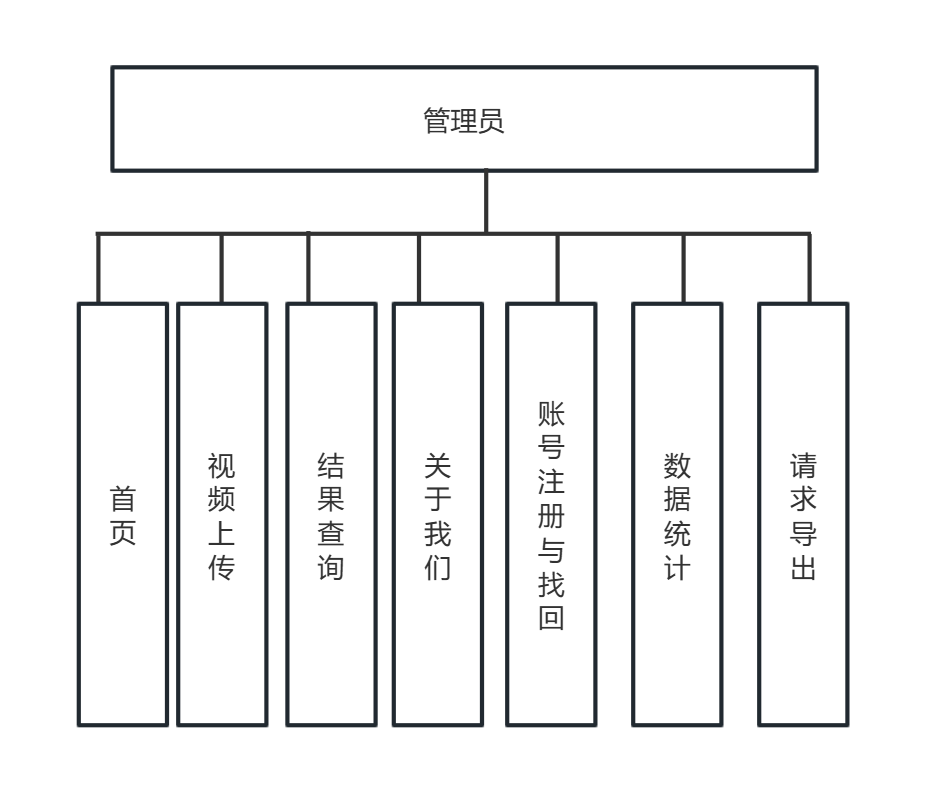
\includegraphics[width=0.4\textwidth]{source/img/admin_uml.png}
    \bicaption{管理员用例图}{Admin Use Case Diagram}
    \label{fig:admin-uml}
\end{figure}

从用例图~\ref{fig:user-uml}和~\ref{fig:admin-uml}分析得出,系统的模块可以划分为:
\begin{itemize}
    \item 首页:作为各个功能模块的入口,完成其他各模块的合理布局;
    \item 用户管理模块:包括用户的注册、登录、注销、密码重置与找回功能;
    \item 任务上传模块:系统的核心功能,完整实现编辑任务上传的全流程;
    \item 结果管理模块:用户在该模块下查询编辑任务的结果,并提供删除、重命名等操作;
    \item 关于我们模块:展示开发者的相关信息;
    \item 数据统计模块:管理员用户在该模块下可以查看用户上传任务的数量、编辑任务的数量、编辑任务的结果数量等数据统计,并导出用户请求数据;
\end{itemize}

\section{模块实现}

本节将介绍系统各个模块的具体实现,包括前端页面、后端接口、数据库设计等。由于首页只作为其余功能模块的载体,
只涉及到前端页面的布局设计,不涉及到与后端的交互;而关于我们模块作为信息展示,仅仅为静态HTML页面,我们也不再详细介绍。
另外,由于各个模块的后端操作都涉及到数据库操作,我们将数据库功能实现单独列出,不再在每个模块中介绍。

\subsection{首页的详细设计与实现}

在前端UI设计中,我们采用Ant Design(Antd)来辅助开发。Antd是一个基于React的UI组件库,提供高质量的React组件,并拥有完整的类型定义文件。

首页的布局采用Antd的Layout组件,使用侧边布局,在左侧放置导航栏以显示各个功能模块,如~\ref{fig:app-dashboard}所示。功能模块间的切换功能通过维护一个全局的
组件状态selectedMenu来实现,导航栏的每一项对应selectedMenu的一个值,检测到用户点击动作时,更新状态为对应的值。

\begin{figure}[ht]
    \centering
    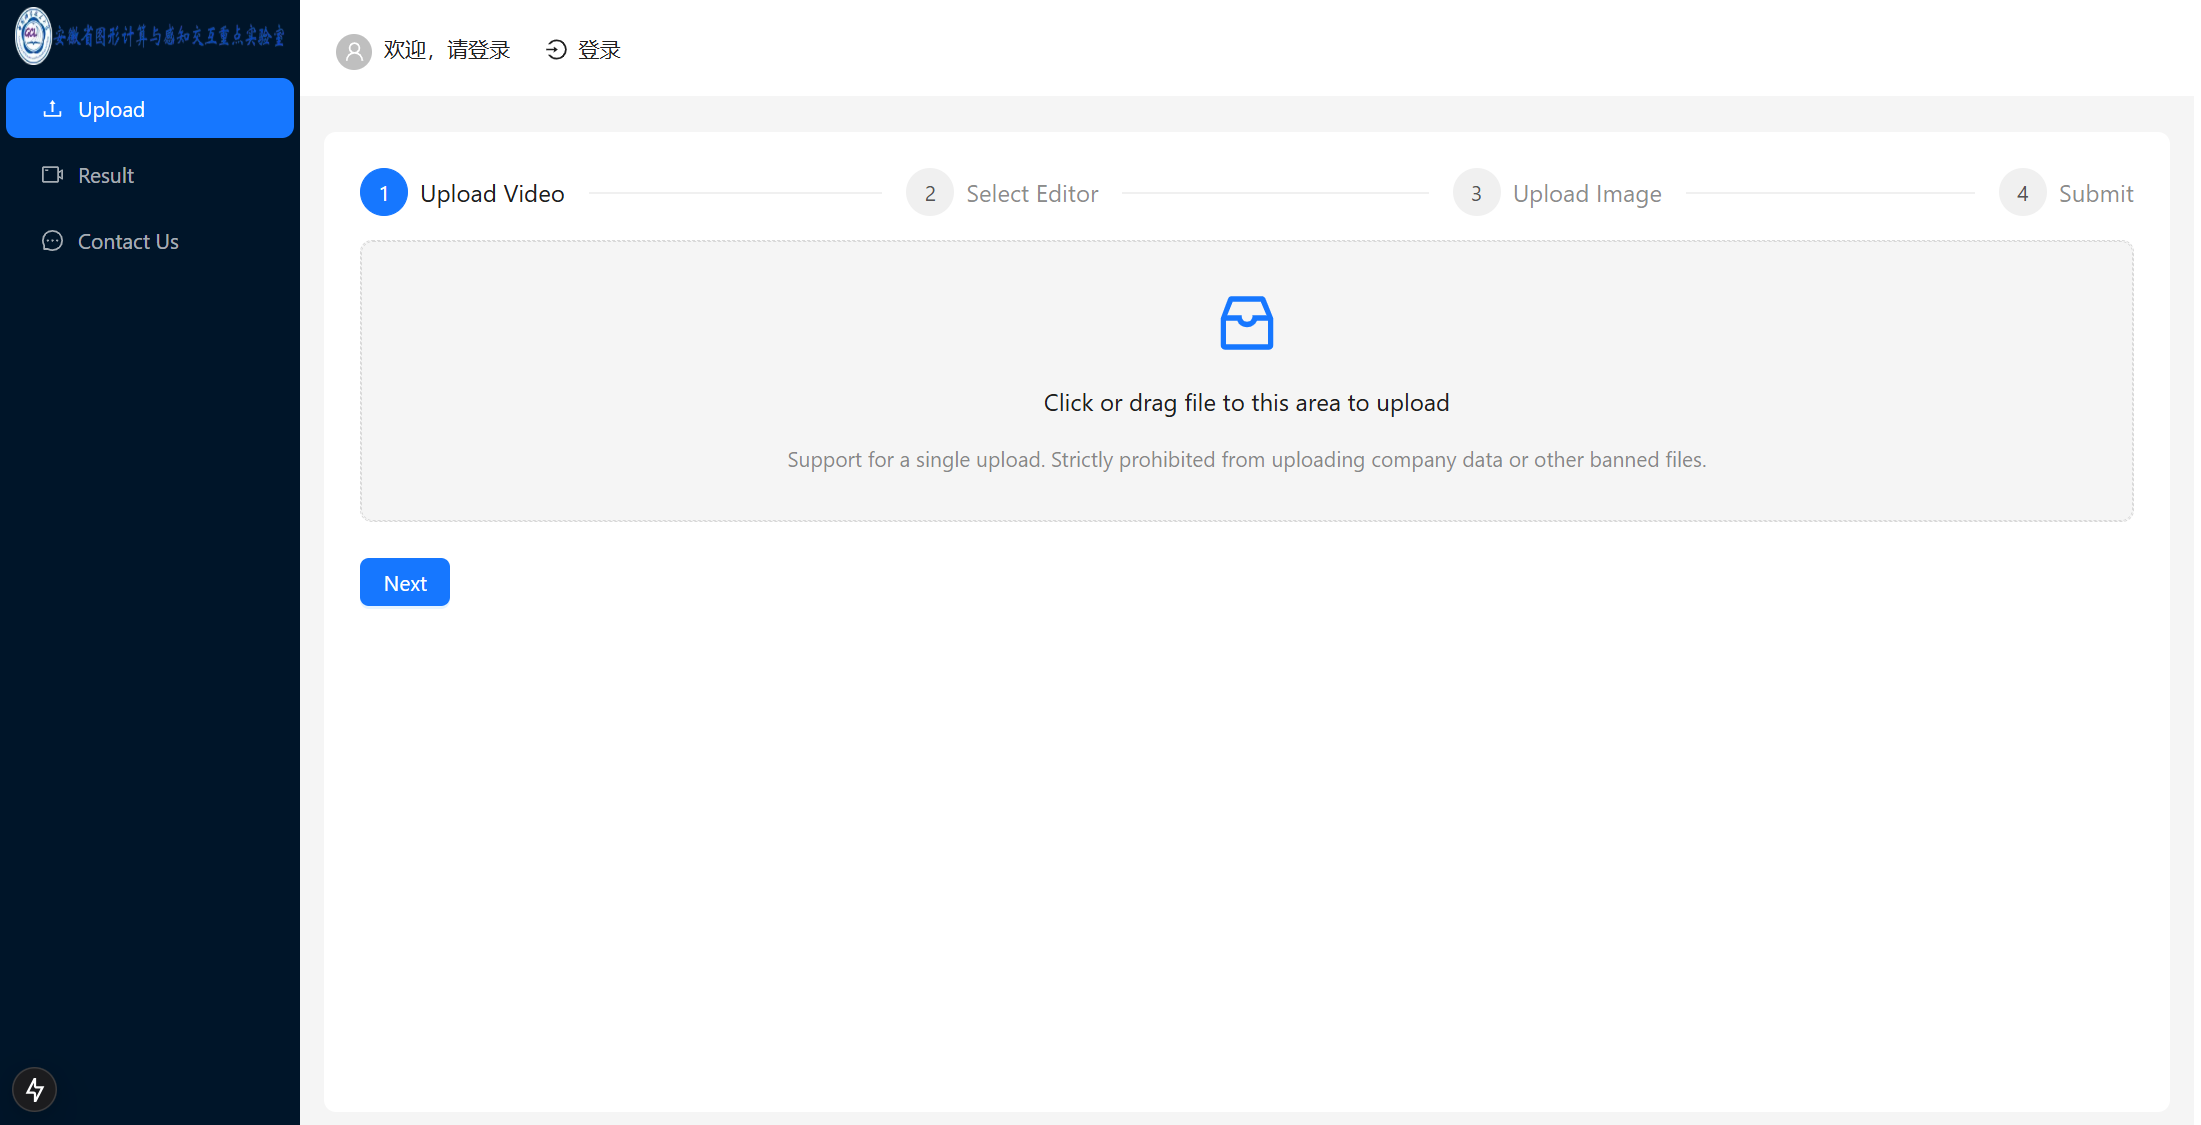
\includegraphics[width=0.8\textwidth]{source/img/app_dashboard.png}
    \bicaption{首页布局}{Home Page Layout}
    \label{fig:app-dashboard}
\end{figure}

为了显示对应模块的内容,我们在Layout组件的Content区域设置条件渲染,根据组件状态selectedMenu的值来渲染不同的组件。
例如selectedMenu的默认值是1,对应任务上传模块,首页默认渲染任务上传组件。此外首页根据用户是否为管理员对导航栏也
进行条件渲染,只有管理员用户才能显示额外的数据统计模块。

\subsection{用户管理的详细设计与实现}

\subsubsection{流程设计}

我们设计的用户登录流程如\ref{fig:login-process}所示,图中包含我们需要实现的三个子流程:用户注册、用户登录与密码找回。
\begin{figure}[ht]
    \centering
    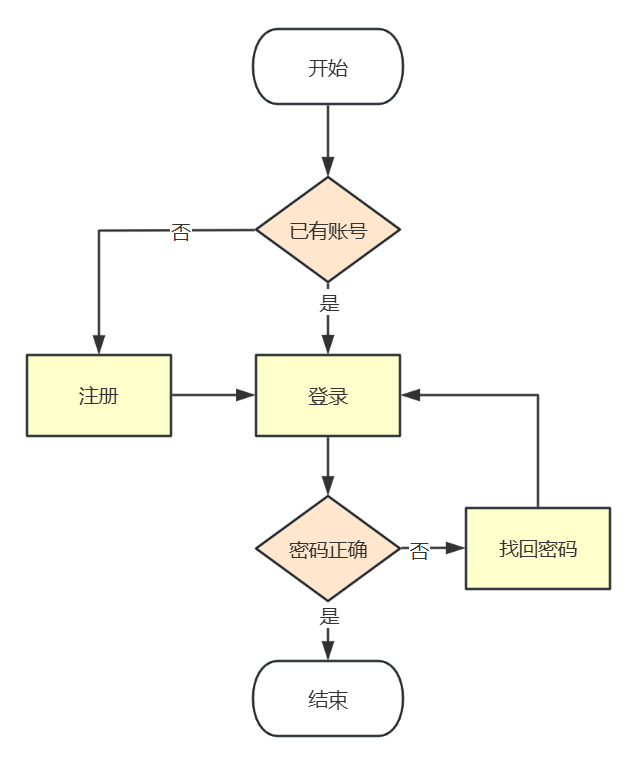
\includegraphics[width=0.4\textwidth]{source/img/login_process.png}
    \bicaption{登录流程图}{Login Process}
    \label{fig:login-process}
\end{figure}

\subsubsection{前端实现}

我们分别为这三个子流程设计了路由页面,并在页面中设置了路由跳转,保证用户页面跳转的双向性。我们使用Antd的Form组件来实现
表单的创建,我们通过设置组件成员的rules属性来设置表单内容检查,包括密码长度、密码复杂度、邮箱是否合法等;
组件中封装的提交按钮通过绑定自定义触发函数以处理提交事件,触发函数的主要逻辑为将后端api需要的数据封装为json格式,
通过axios发送post请求到后端,并处理返回结果。

由于系统中结果查询、上传限制查询等功能都需要使用用户信息,我们又无法频繁地要求用户录入信息,因此在登录流程中,
我们需要维护全局的用户状态以供其他模块使用。为了携带cookies信息到全局,我们选择了使用localStorage来存储用户信息,
在用户登录成功后,我们存储全局的用户信息并设置过期时间,在用户登出时,我们清除全局的用户信息。当其他模块需要使用
用户信息时,只需要从localStorage中解析出所需要的字段即可。

密码找回功能由于涉及到敏感信息,存在安全风险,因此我们设计了两步找回方式。我们需要用户输入邮箱,验证邮箱验证码通过后
自动跳转到密码重置页面,并由后端返回token,用户在重置密码时需要携带token,后端验证token后才能重置密码。这种设计可以防止
用户直接进入重置密码路由对数据库进行攻击,相比于临时生成动态路由,避免了动态路由规则被暴力破解的风险。

\subsubsection{后端实现}

后端主要实现的功能包括验证邮件发送、token生成与验证。

\subsection{任务管理的详细设计与实现}

\subsubsection{任务上传}

根据视频编辑算法的输入,需要用户提供视频、编辑提示类型与对应的提示内容,并提供邮箱以获取编辑结果。上传流程如\ref{fig:upload_process}所示。
\begin{figure}[ht]
    \centering
    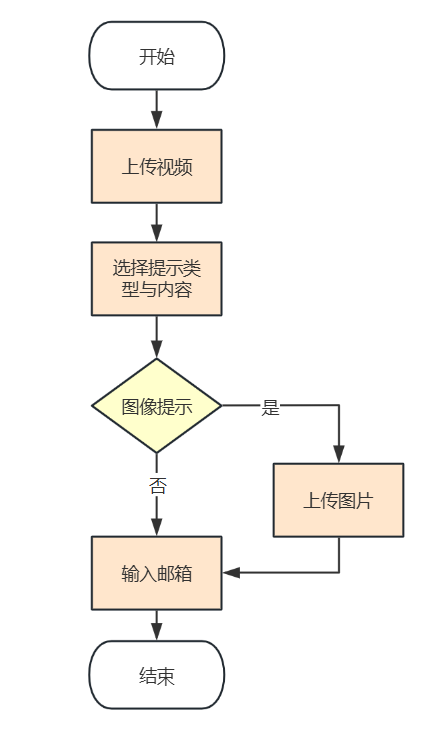
\includegraphics[width=0.3\textwidth]{source/img/edit_process.png}
    \bicaption{上传流程图}{Upload Process}
    \label{fig:upload_process}
\end{figure}

\subsection{结果管理的详细设计与实现}

\subsubsection{结果管理}

用户在结果查询界面可以查看自己上传的任务进度与结果,系统也支持任务重命名与删除,同时在任务处理完成后会自动生成略缩图,方便用户预览结果。

\subsection{数据统计的详细设计与实现}


\subsection{数据库功能实现}

我们使用PyMySQL作为Flask框架下的MySQL数据库驱动,受到SQLAlchemy等ORM驱动框架将数据库操作封装为对象方法的启发,我们
将常用的数据库操作封装为函数,以方便在Flask应用中调用。

我们还在数据库中添加了连接池设计,以提高数据库连接的效率。由于MySQL数据库是通过TCP协议进行通信的,因此每次建立连接都需要进行三次握手,
以实现TCP的可靠传输;而建立TCP连接后数据库还需要传输认证包用于用户验证,因此数据库连接的建立是一个相对耗时的操作。我们采用的连接池设计
通过维护一定数量的数据库连接,在需要时直接从连接池中获取数据库连接,避免了频繁建立数据库连接带来的性能问题。

\subsection{安全控制设计}

在系统构建的过程中,安全控制是一个至关重要的方面。为了防止未经授权的访问和操作,我们需要用户在登录状态下进行操作,这涉及到对用户信息与数据的
加密保护;我们也需要限制用户的操作行为,以防止用户的恶意操作;另外为了保证服务器的安全性,我们也需要系统部署过程中的安全措施。

\subsubsection{用户信息与数据加密}

我们将用户信息存储在数据库中,包括用户名、密码、邮箱等敏感信息。为了保证用户信息的安全性,我们对输入信息加密后存储。
我们使用密钥派生函数(Key Derivation Function, KDF)将用户提供的弱密码根据一些额外参数生成强密码,具体来说,
我们将用户的密码与给定的盐值(salt)连接起来,利用SHA256等加密函数经过多轮迭代得到最终的密码哈希值。由于哈希函数
具有单向性,我们无法通过哈希值反推原始密码,因此在验证用户密码时,我们只能重新计算哈希值并与存储的哈希值进行比较。

这种加密方式通过刻意使密钥派生的速度变慢,从而增加暴力破解的难度;同时由于不同密钥对应的盐值不同,确保了即使相同的密码
也会产生不同的哈希值,能够抵抗彩虹表攻击。

\subsubsection{用户行为限制}

为了防止用户恶意操作,如短时间大量上传文件、大量提交任务等,我们对用户行为做出一定的限制。具体包括:
\begin{itemize}
    \item 用户上传的文件在没有提交任务时被设置为一小时过期,未使用的文件达上限时拒绝用户的上传行为;
    \item 由于任务处理需要一定的时间,我们限制用户在处理的任务数量上限,超过限制则拒绝用户提交任务;
\end{itemize}
这些限制的具体实现通过MySQL数据库的触发器和在后台运行的定时任务完成。在插入数据时过期时间被设置为一小时后,当有任务使用到
对应文件时,UsedByProjectID字段外键引用任务ID;任务被删除时外键引用设置为NULL,触发器检测到后将时间设置为当前时间,文件过期。
后台的定时任务通过查询文件的过期时间字段来定时删除过期的文件。

\subsubsection{部署安全措施}

为了保证服务器的安全性,我们采取了以下措施:
\begin{itemize}
    \item 限制服务器中部署用户组的权限,避免系统文件遭到篡改;
    \item 文件传输使用HTTPS协议传输,通过SSL/TSL协议建立加密的传输通道
    \item 服务器部署在内网,限制外部访问,在网关上设置防火墙。
\end{itemize}